\documentclass{article}
\usepackage{amsmath}
\usepackage{amsfonts}
\usepackage{amssymb}
\usepackage{graphicx}
\usepackage{hyperref}

\begin{document}

\title{C H A P T E R 1\\Angle Chasing}
\maketitle

\section*{Morpheus in The Matrix}
This is your last chance. After this, there is no turning back. You take the blue pill—the story ends, you wake up in your bed and believe whatever you want to believe. You take the red pill—you stay in Wonderland and I show you how deep the rabbit-hole goes.

\section{Angle Chasing}
Angle chasing is one of the most fundamental skills in olympiad geometry. For that reason, we dedicate the entire first chapter to fully developing the technique.

\subsection{Triangles and Circles}
Consider the following example problem, illustrated in Figure \ref{fig:example}.

\begin{figure}
    \centering
    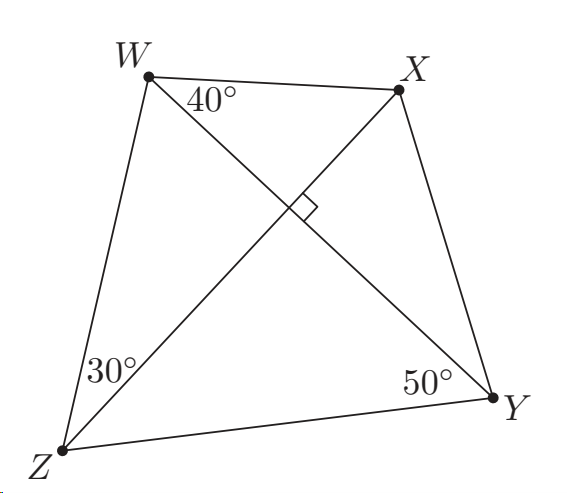
\includegraphics[width=0.5\linewidth]{Image.png}
    \caption{Enter Caption}
    \label{fig:enter-label}
\end{figure}

\textbf{Example 1.1.} In quadrilateral WXYZ with perpendicular diagonals (as in Figure \ref{fig:example}), we are given \( \angle WZX = 30^\circ \), \( \angle XWY = 40^\circ \), and \( \angle WYZ = 50^\circ \).

\begin{enumerate}
    \item[(a)] Compute \( \angle Z \).
    \item[(b)] Compute \( \angle X \).
\end{enumerate}

Figure 1.1A. Given these angles, which other angles can you compute? You probably already know the following fact:

\begin{figure}
    \centering
    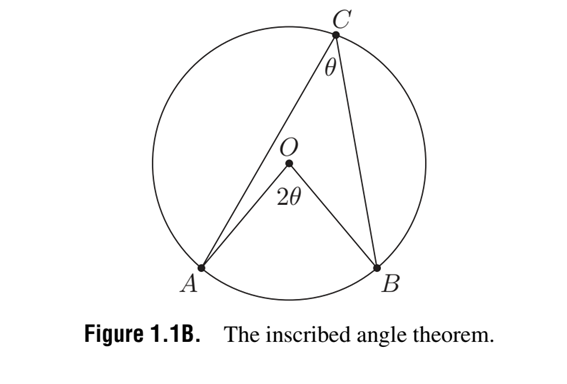
\includegraphics[width=0.5\linewidth]{Image2.png}
    \caption{Enter Caption}
    \label{fig:enter-label}
\end{figure}


Figure 1.1B. The inscribed angle theorem.

We need some way to use the condition \( AO = BO = CO \). How do we do so? Using isosceles triangles, roughly the only way we know how to convert lengths into angles. Because \( AO = CO \), we know that \( \angle OAC = \angle OCA = \alpha \). How does this help? Using Proposition 1.2 gives

\[
\angle AOC = 180^\circ - (\angle OAC + \angle OCA) = 180^\circ - 2\alpha.
\]

Now we do exactly the same thing with \( B \). We can derive

\[
\angle BOC = 180^\circ - 2\beta.
\]

Therefore,

\[
\angle AOB = 360^\circ - (\angle AOC + \angle BOC) = 360^\circ - (360^\circ - 2\alpha - 2\beta) = 2\theta
\]

and we are done.

We can also get information about the centers defined in Section 0.2. For example, recall the incenter is the intersection of the angle bisectors.

\end{document}